\chapter{RRD Trending Graph FAQ}
\label{chap:hobbitgraph}


This FAQ is a collection of Trending Graphs create Hobbit Server.

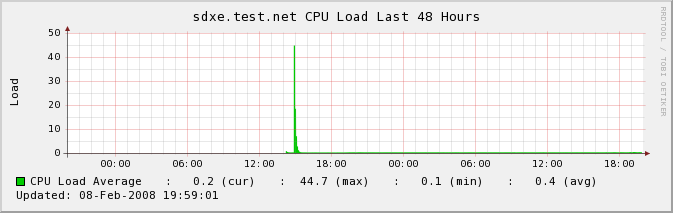
\includegraphics[scale=0.6]{./hobbitgraph.png} 


\begin{figure}[htb]
  \centering
  \grafix{hobbitgraph}
  \caption{CPU load }
  \label{fig:cpu:load}
\end{figure}


\section{Round Robin Database(RRD) }
\label{sec:style}

Hobbit use \hbgraph{RRD} as database backend to to store metrics data.


\interaction{template.simple.normal}

This is somewhat informative, but it takes up a lot of space---five
lines of output per changeset.  The \texttt{compact} style reduces
this to three lines, presented in a sparse manner.

\interaction{template.simple.compact}

The \texttt{changelog} style hints at the expressive power of
Mercurial's templating engine.  This style attempts to follow the GNU
Project's changelog guidelines\cite{web:changelog}.

\interaction{template.simple.changelog}

You will not be shocked to learn that Mercurial's default output style
is named \texttt{default}.

\section{What is RRD ?}

You can modify the output style that Mercurial will use for every
command by editing your \hgrc\ file, naming the style you would
prefer to use.

\begin{codesample2}
  [ui]
  style = compact
\end{codesample2}

If you write a style of your own, you can use it by either providing
the path to your style file, or copying your style file into a
location where Mercurial can find it (typically the \texttt{templates}
subdirectory of your Mercurial install directory).

\section{Reading Hobbit Graphs}

All of Mercurial's ``\texttt{log}-like'' commands let you use styles
and templates: \hgcmd{incoming}, \hgcmd{log}, \hgcmd{outgoing}, and
\hgcmd{tip}.

As I write this manual, these are so far the only commands that
support styles and templates.  Since these are the most important
commands that need customisable output, there has been little pressure
from the Mercurial user community to add style and template support to
other commands.

\section{Metrics Reading }

At its simplest, a Mercurial template is a piece of text.  Some of the
text never changes, while other parts are \emph{expanded}, or replaced
with new text, when necessary.


\section{What is RRD ?}


Before we continue, let's look again at a simple example of
Mercurial's normal output.

\interaction{template.simple.normal}

Now, let's run the same command, but using a template to change its
output.

\interaction{template.simple.simplest}

The example above illustrates the simplest possible template; it's
just a piece of static text, printed once for each changeset.  The
\hgopt{log}{--template} option to the \hgcmd{log} command tells
Mercurial to use the given text as the template when printing each
changeset.

Notice that the template string above ends with the text
``\Verb+\n+''.  This is an \emph{escape sequence}, telling Mercurial
to print a newline at the end of each template item.  If you omit this
newline, Mercurial will run each piece of output together.  See
section~\ref{sec:template:escape} for more details of escape sequences.

A template that prints a fixed string of text all the time isn't very
useful; let's try something a bit more complex.

\interaction{template.simple.simplesub}

As you can see, the string ``\Verb+{desc}+'' in the template has been
replaced in the output with the description of each changeset.  Every
time Mercurial finds text enclosed in curly braces (``\texttt{\{}''
and ``\texttt{\}}''), it will try to replace the braces and text with
the expansion of whatever is inside.  To print a literal curly brace,
you must escape it, as described in section~\ref{sec:template:escape}.

\section{Common template keywords}
\label{sec:template:keyword}

You can start writing simple templates immediately using the keywords
below.

\begin{itemize}
\item[\tplkword{author}] String.  The unmodified author of the changeset.
\item[\tplkword{branches}] String.  The name of the branch on which
  the changeset was committed.  Will be empty if the branch name was
  \texttt{default}.
\item[\tplkword{date}] Date information.  The date when the changeset
  was committed.  This is \emph{not} human-readable; you must pass it
  through a filter that will render it appropriately.  See
  section~\ref{sec:template:filter} for more information on filters.
  The date is expressed as a pair of numbers.  The first number is a
  Unix UTC timestamp (seconds since January 1, 1970); the second is
  the offset of the committer's timezone from UTC, in seconds.
\item[\tplkword{desc}] String.  The text of the changeset description.
\item[\tplkword{files}] List of strings.  All files modified, added, or
  removed by this changeset.
\item[\tplkword{file\_adds}] List of strings.  Files added by this
  changeset.
\item[\tplkword{file\_dels}] List of strings.  Files removed by this
  changeset.
\item[\tplkword{node}] String.  The changeset identification hash, as a
  40-character hexadecimal string.
\item[\tplkword{parents}] List of strings.  The parents of the
  changeset.
\item[\tplkword{rev}] Integer.  The repository-local changeset revision
  number.
\item[\tplkword{tags}] List of strings.  Any tags associated with the
  changeset.
\end{itemize}

A few simple experiments will show us what to expect when we use these
keywords; you can see the results in
figure~\ref{fig:template:keywords}.

\begin{figure}
  \interaction{template.simple.keywords}
  \caption{Template keywords in use}
  \label{fig:template:keywords}
\end{figure}

As we noted above, the date keyword does not produce human-readable
output, so we must treat it specially.  This involves using a
\emph{filter}, about which more in section~\ref{sec:template:filter}.

\interaction{template.simple.datekeyword}

\section{Escape sequences}
\label{sec:template:escape}

Mercurial's templating engine recognises the most commonly used escape
sequences in strings.  When it sees a backslash (``\Verb+\+'')
character, it looks at the following character and substitutes the two
characters with a single replacement, as described below.

\begin{itemize}
\item[\Verb+\textbackslash\textbackslash+] Backslash, ``\Verb+\+'',
  ASCII~134.
\item[\Verb+\textbackslash n+] Newline, ASCII~12.
\item[\Verb+\textbackslash r+] Carriage return, ASCII~15.
\item[\Verb+\textbackslash t+] Tab, ASCII~11.
\item[\Verb+\textbackslash v+] Vertical tab, ASCII~13.
\item[\Verb+\textbackslash \{+] Open curly brace, ``\Verb+{+'', ASCII~173.
\item[\Verb+\textbackslash \}+] Close curly brace, ``\Verb+}+'', ASCII~175.
\end{itemize}

As indicated above, if you want the expansion of a template to contain
a literal ``\Verb+\+'', ``\Verb+{+'', or ``\Verb+{+'' character, you
must escape it.

\section{Filtering keywords to change their results}
\label{sec:template:filter}

Some of the results of template expansion are not immediately easy to
use.  Mercurial lets you specify an optional chain of \emph{filters}
to modify the result of expanding a keyword.  You have already seen a
common filter, \tplkwfilt{date}{isodate}, in action above, to make a
date readable.

Below is a list of the most commonly used filters that Mercurial
supports.  While some filters can be applied to any text, others can
only be used in specific circumstances.  The name of each filter is
followed first by an indication of where it can be used, then a
description of its effect.

\begin{itemize}
\item[\tplfilter{addbreaks}] Any text. Add an XHTML ``\Verb+<br/>+''
  tag before the end of every line except the last.  For example,
  ``\Verb+foo\nbar+'' becomes ``\Verb+foo<br/>\nbar+''.
\item[\tplkwfilt{date}{age}] \tplkword{date} keyword.  Render the
  age of the date, relative to the current time.  Yields a string like
  ``\Verb+10 minutes+''.
\item[\tplfilter{basename}] Any text, but most useful for the
  \tplkword{files} keyword and its relatives.  Treat the text as a
  path, and return the basename. For example, ``\Verb+foo/bar/baz+''
  becomes ``\Verb+baz+''.
\item[\tplkwfilt{date}{date}] \tplkword{date} keyword.  Render a date
  in a similar format to the Unix \tplkword{date} command, but with
  timezone included.  Yields a string like
  ``\Verb+Mon Sep 04 15:13:13 2006 -0700+''.
\item[\tplkwfilt{author}{domain}] Any text, but most useful for the
  \tplkword{author} keyword.  Finds the first string that looks like
  an email address, and extract just the domain component.  For
  example, ``\Verb+Bryan O'Sullivan <bos@serpentine.com>+'' becomes
  ``\Verb+serpentine.com+''.
\item[\tplkwfilt{author}{email}] Any text, but most useful for the
  \tplkword{author} keyword.  Extract the first string that looks like
  an email address.  For example,
  ``\Verb+Bryan O'Sullivan <bos@serpentine.com>+'' becomes
  ``\Verb+bos@serpentine.com+''.
\item[\tplfilter{escape}] Any text.  Replace the special XML/XHTML
  characters ``\Verb+&+'', ``\Verb+<+'' and ``\Verb+>+'' with
  XML entities.
\item[\tplfilter{fill68}] Any text.  Wrap the text to fit in 68
  columns.  This is useful before you pass text through the
  \tplfilter{tabindent} filter, and still want it to fit in an
  80-column fixed-font window.
\item[\tplfilter{fill76}] Any text.  Wrap the text to fit in 76
  columns.
\item[\tplfilter{firstline}] Any text.  Yield the first line of text,
  without any trailing newlines.
\item[\tplkwfilt{date}{hgdate}] \tplkword{date} keyword.  Render the
  date as a pair of readable numbers.  Yields a string like
  ``\Verb+1157407993 25200+''.
\item[\tplkwfilt{date}{isodate}] \tplkword{date} keyword.  Render the
  date as a text string in ISO~8601 format.  Yields a string like
  ``\Verb+2006-09-04 15:13:13 -0700+''.
\item[\tplfilter{obfuscate}] Any text, but most useful for the
  \tplkword{author} keyword.  Yield the input text rendered as a
  sequence of XML entities.  This helps to defeat some particularly
  stupid screen-scraping email harvesting spambots.
\item[\tplkwfilt{author}{person}] Any text, but most useful for the
  \tplkword{author} keyword.  Yield the text before an email address.
  For example, ``\Verb+Bryan O'Sullivan <bos@serpentine.com>+''
  becomes ``\Verb+Bryan O'Sullivan+''.
\item[\tplkwfilt{date}{rfc822date}] \tplkword{date} keyword.  Render a
  date using the same format used in email headers.  Yields a string
  like ``\Verb+Mon, 04 Sep 2006 15:13:13 -0700+''.
\item[\tplkwfilt{node}{short}] Changeset hash.  Yield the short form
  of a changeset hash, i.e.~a 12-byte hexadecimal string.
\item[\tplkwfilt{date}{shortdate}] \tplkword{date} keyword.  Render
  the year, month, and day of the date.  Yields a string like
  ``\Verb+2006-09-04+''.
\item[\tplfilter{strip}] Any text.  Strip all leading and trailing
  whitespace from the string.
\item[\tplfilter{tabindent}] Any text.  Yield the text, with every line
  except the first starting with a tab character.
\item[\tplfilter{urlescape}] Any text.  Escape all characters that are
  considered ``special'' by URL parsers.  For example, \Verb+foo bar+
  becomes \Verb+foo%20bar+.
\item[\tplkwfilt{author}{user}] Any text, but most useful for the
  \tplkword{author} keyword.  Return the ``user'' portion of an email
  address.  For example,
  ``\Verb+Bryan O'Sullivan <bos@serpentine.com>+'' becomes
  ``\Verb+bos+''.
\end{itemize}

\begin{figure}
  \interaction{template.simple.manyfilters}
  \caption{Template filters in action}
  \label{fig:template:filters}
\end{figure}

\begin{note}
  If you try to apply a filter to a piece of data that it cannot
  process, Mercurial will fail and print a Python exception.  For
  example, trying to run the output of the \tplkword{desc} keyword
  into the \tplkwfilt{date}{isodate} filter is not a good idea.
\end{note}

\section{Combining filters}

It is easy to combine filters to yield output in the form you would
like.  The following chain of filters tidies up a description, then
makes sure that it fits cleanly into 68 columns, then indents it by a
further 8~characters (at least on Unix-like systems, where a tab is
conventionally 8~characters wide).

\interaction{template.simple.combine}

Note the use of ``\Verb+\t+'' (a tab character) in the template to
force the first line to be indented; this is necessary since
\tplkword{tabindent} indents all lines \emph{except} the first.

Keep in mind that the order of filters in a chain is significant.  The
first filter is applied to the result of the keyword; the second to
the result of the first filter; and so on.  For example, using
\Verb+fill68|tabindent+ gives very different results from
\Verb+tabindent|fill68+.


\section{From templates to styles}

A command line template provides a quick and simple way to format some
output.  Templates can become verbose, though, and it's useful to be
able to give a template a name.  A style file is a template with a
name, stored in a file.

More than that, using a style file unlocks the power of Mercurial's
templating engine in ways that are not possible using the command line
\hgopt{log}{--template} option.

\section{The simplest of style files}

Our simple style file contains just one line:

\interaction{template.simple.rev}

This tells Mercurial, ``if you're printing a changeset, use the text
on the right as the template''.

\section{Style file syntax}

The syntax rules for a style file are simple.

\begin{itemize}
\item The file is processed one line at a time.

\item Leading and trailing white space are ignored.

\item Empty lines are skipped.

\item If a line starts with either of the characters ``\texttt{\#}'' or
  ``\texttt{;}'', the entire line is treated as a comment, and skipped
  as if empty.

\item A line starts with a keyword.  This must start with an
  alphabetic character or underscore, and can subsequently contain any
  alphanumeric character or underscore.  (In regexp notation, a
  keyword must match \Verb+[A-Za-z_][A-Za-z0-9_]*+.)

\item The next element must be an ``\texttt{=}'' character, which can
  be preceded or followed by an arbitrary amount of white space.

\item If the rest of the line starts and ends with matching quote
  characters (either single or double quote), it is treated as a
  template body.

\item If the rest of the line \emph{does not} start with a quote
  character, it is treated as the name of a file; the contents of this
  file will be read and used as a template body.
\end{itemize}

\section{Style files by example}

To illustrate how to write a style file, we will construct a few by
example.  Rather than provide a complete style file and walk through
it, we'll mirror the usual process of developing a style file by
starting with something very simple, and walking through a series of
successively more complete examples.

\section{Identifying mistakes in style files}

If Mercurial encounters a problem in a style file you are working on,
it prints a terse error message that, once you figure out what it
means, is actually quite useful.

\interaction{template.svnstyle.syntax.input}

Notice that \filename{broken.style} attempts to define a
\texttt{changeset} keyword, but forgets to give any content for it.
When instructed to use this style file, Mercurial promptly complains.

\interaction{template.svnstyle.syntax.error}

This error message looks intimidating, but it is not too hard to
follow.

\begin{itemize}
\item The first component is simply Mercurial's way of saying ``I am
  giving up''.
  \begin{codesample4}
    \textbf{abort:} broken.style:1: parse error
  \end{codesample4}

\item Next comes the name of the style file that contains the error.
  \begin{codesample4}
    abort: \textbf{broken.style}:1: parse error
  \end{codesample4}

\item Following the file name is the line number where the error was
  encountered.
  \begin{codesample4}
    abort: broken.style:\textbf{1}: parse error
  \end{codesample4}

\item Finally, a description of what went wrong.
  \begin{codesample4}
    abort: broken.style:1: \textbf{parse error}
  \end{codesample4}
  The description of the problem is not always clear (as in this
  case), but even when it is cryptic, it is almost always trivial to
  visually inspect the offending line in the style file and see what
  is wrong.
\end{itemize}

\section{Uniquely identifying a repository}

If you would like to be able to identify a Mercurial repository
``fairly uniquely'' using a short string as an identifier, you can
use the first revision in the repository.
\interaction{template.svnstyle.id} 
This is not guaranteed to be unique, but it is nevertheless useful in
many cases.
\begin{itemize}
\item It will not work in a completely empty repository, because such
  a repository does not have a revision~zero.
\item Neither will it work in the (extremely rare) case where a
  repository is a merge of two or more formerly independent
  repositories, and you still have those repositories around.
\end{itemize}
Here are some uses to which you could put this identifier:
\begin{itemize}
\item As a key into a table for a database that manages repositories
  on a server.
\item As half of a \{\emph{repository~ID}, \emph{revision~ID}\} tuple.
  Save this information away when you run an automated build or other
  activity, so that you can ``replay'' the build later if necessary.
\end{itemize}

\section{Mimicking Subversion's output}

Let's try to emulate the default output format used by another
revision control tool, Subversion.
\interaction{template.svnstyle.short}

Since Subversion's output style is fairly simple, it is easy to
copy-and-paste a hunk of its output into a file, and replace the text
produced above by Subversion with the template values we'd like to see
expanded.
\interaction{template.svnstyle.template}

There are a few small ways in which this template deviates from the
output produced by Subversion.
\begin{itemize}
\item Subversion prints a ``readable'' date (the ``\texttt{Wed, 27 Sep
    2006}'' in the example output above) in parentheses.  Mercurial's
  templating engine does not provide a way to display a date in this
  format without also printing the time and time zone.
\item We emulate Subversion's printing of ``separator'' lines full of
  ``\texttt{-}'' characters by ending the template with such a line.
  We use the templating engine's \tplkword{header} keyword to print a
  separator line as the first line of output (see below), thus
  achieving similar output to Subversion.
\item Subversion's output includes a count in the header of the number
  of lines in the commit message.  We cannot replicate this in
  Mercurial; the templating engine does not currently provide a filter
  that counts the number of items it is passed.
\end{itemize}
It took me no more than a minute or two of work to replace literal
text from an example of Subversion's output with some keywords and
filters to give the template above.  The style file simply refers to
the template.
\interaction{template.svnstyle.style}

We could have included the text of the template file directly in the
style file by enclosing it in quotes and replacing the newlines with
``\texttt{n}'' sequences, but it would have made the style file too
difficult to read.  Readability is a good guide when you're trying to
decide whether some text belongs in a style file, or in a template
file that the style file points to.  If the style file will look too
big or cluttered if you insert a literal piece of text, drop it into a
template instead.

%%% Local Variables: 
%%% mode: latex
%%% TeX-master: "00book"
%%% End: 
